\documentclass[fleqn]{jbook}
\usepackage{physpub}

\begin{document}

\begin{question}{$B650i(B $B1Q8l(B}{}

\begin{subquestions}
\SubQuestion
  $B0J2<$NJ8>O$rFI$_!"2<@~It(B(1)$B!A(B(6)$B$rOBLu$;$h!#(B
\baselineskip=12pt

  $B!!(B\underlineeng{(1)A scientific model begins with a real physical
  object or system, replaces the original object with a simpler object,
  and then represents the simplified object with equations describing
  its behavior.}
  \underlineeng{(2)Like a toy boat, a scientific model is a
  scaled-down version of a physical system, missing some parts of the
  original.}
  \underlineeng{(3)Deciding what parts should be left out requires
  judgement and skill.}
  \underlineeng{(4)The omission of essential features makes the
  model worthless.}
  \underlineeng{(5)On the other hand, if nothing is left out, no
  simplification has been made.}
  In making a model of a swinging pendulum, for example, we might at
  first try to include the detailed shape of the weight at the end,
  the density and pressure of the air in the room, and so on. Finding
  such a description too complex to manage, we could replace the
  weight by a round ball neglect the air completely. This much simpler
  system, in fact, behaves almost exactly like the original. If, on
  the other hand, we left out gravity, the resulting theoretical
  pendulum would not swing back and forth.
  \underlineeng{(6)By solving the equations of a model,
  predictions can be made about the original physical system and then
  tested.}

  \rightline{--- quoted from `Origin' by A. Lightman and R. Brawer}
\baselineskip=15pt

\SubQuestion
  $B0J2<$N3FJ8>O$O(B,$P$$B$H(B$I$$B$H$N4X78$K4X$9$k$"$k<B837k2L$K$D$$$F@bL@$7$?(B
  $B$b$N$G$"$k!#3FJ8$r1QLu$;$h!#2rEz$G$O!"(B$P$,$I$$B$O$=$N$^$^$G$h$$!#(B
%
  \begin{subsubquestions}%
  \SubSubQuestion
    $B$3$l$^$G$N8&5f$K$*$$$F2f!9$O!"(B$P$$B$O29EY$K0MB8$7$J$$$H2>Dj$7$F!"(B
    $B$"$kFCDj$N29EY$G(B$I$$B$N4X?t$H$7$F(B$P$$B$rB,Dj$7$F$$$?!#(B
  \SubSubQuestion
    $B$3$N2>Dj$NBEEv@-$r8!F$$9$k$?$a$KK\<B83$G$O!"MM!9$J29EY$G(B$P$$B$r(B
    $BB,Dj$7$?!#(B
  \SubSubQuestion
    $B?^(B1$B$G!"9u4](B(filled circles)$B$O(B$25\degC$$B!"9u;03Q(B(filled triangles)$B$O(B
    $20\degC$$B!"Gr%L%-$N;M3Q(B(open squares)$B$O(B$15\degC$$B$K$*$1$kB,Dj7k2L$r(B
    $B<($9!#(B\\
  \parbox[t]{80mm}{
  \SubSubQuestion
    $ 25\degC $$B$K$*$$$F!"(B$I$$B$,(B$300\mu\Unit{mol\,m^{-2}s^{-1}}$$B0J2<$G$O(B $I$$B$NA}2C$KH<$C$F(B$P$$B$OD>@~E*$KA}2C$7!"(B$300\Unit{\mu mol\,m^{-2}s^{-1}}$$B0J>e$G$O0lDj$NCM(B$0.4\Unit{\mu mol\,O_2 mg^{-1}h^{-1}}$$B$H$J$k!#(B
  \SubSubQuestion
    $P$$B$N0lDjCM$O!"(B$15\degC$$B$G$O(B$25\degC$$B$N(B4$BJ,$N(B1$B$G$"$k!#(B
  \SubSubQuestion
    $P$$B$,0lDj$NCM$KC#$9$k$H$-$N(B$I$$B$NCM$O29EY$NDc2<$KH<$C$F>.$5$/$J$k!#(B
  \SubSubQuestion
    $B0lJ}!"(B$I$$B$,(B0$B$N;~$N(B$P$$B$NCM$O!"29EY$,9b$$$[$I>.$5$$!#(B
  \SubSubQuestion
    $B$3$&$7$?7k2L$O!"(B$P$$B$,29EY$K0MB8$7$J$$$H$$$&2>Dj$KH?$9$k!#(B
  \SubSubQuestion
    $B$h$j9b29$G$N(B$P$$B$H(B$I$$B$H$N4X78$K$D$$$F!":#8e$5$i$K<B83$,I,MW$G$"$k!#(B
  }\parbox[t]{80mm}{
  \begin{center}
    \mbox{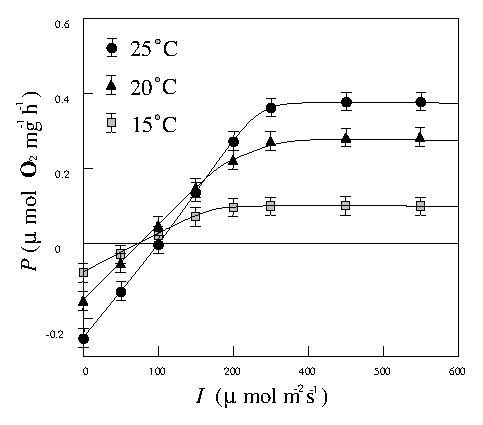
\includegraphics[clip]{1995engl-1.eps}}
  \end{center}}
  \end{subsubquestions}

\newpage
\SubQuestion

  $B0J2<$NJ8>O$rFI$_!"J8Cf$NFbMF$K1h$C$F!"@_Ld$KF|K\8l$GEz$($J$5$$!#(B
  $B3F@_Ld$X$N2rEz$NFbMF$O!"8_$$$K=EJ#$9$kItJ,$,$"$C$F$bNI$$!#(B
\baselineskip=12pt

  $B!!(BOne way of generating ideas is just to generate them---that is,
  to talk out or write down what ever comes into your head about the
  topic you want to write about. Don't worry about whether the ideas
  are good or adequate or complete; just get them down. The purpose
  of brainstorming is to provide yourself with some notes that you
  can use to further stimulate your thinking and organizing. If you
  feel intimidated by a blank page, you might try talking into a tape
  recorder about your topic and then listening to what you've said
  and writing down the good ideas that are there.

  $B!!(BBrainstorming is a very intuitive process. You just follow your
  ideas wherever they lead and take notes to record your mental
  journey. It's important that you not censor an idea before it has a
  chance to flower, but just generate it. Evaluation and organization
  of the ideas will come later, but you can't evaluate or organize
  something that isn't there.

  $B!!(BBrainstorming is often best done in collaboration with other
  people. By ``bouncing ideas'' off of others, you can stimulate their
  thinking and get them to produce ideas of their own. As with any
  kind of brainstorming, the important thing is not to evaluate or
  criticize ideas but just to generate them.

  $B!!(BIf you are collaborating with others who are not always in your
  room or building, you might see if you and your collaborators can
  collaborate via computer. To do this you will all need access to
  computers on a network with connects each computer.
%
  \begin{flushright}
  ---from ``Technical Writing and Professional Communication%
     For Nonnative Speakers of English'',\\
     2nd edition, by T.N.Huckin and L.A.Olsen
  \end{flushright}
%
\begin{list}{}{\itemindent=0mm \labelwidth=28mm \leftmargin=28mm
\topsep=0mm \itemsep=0mm \parsep=0mm}
\item[intimidate:(verb)\hfill]
frighten somebody (in order to make him do something);
{\it intimidate a witness into silence}, e.g. by threating him.

\item[intuitive:(adj.)\hfill]
(1) of or coming from intuition;
{\it intuitive feeling}\\
(2)possessing intuition;
{\it Are women more intuitive than men?}

\item[intuition:(noun)\hfill]
(1) (power of)understanding things immediately, without the need for
conscious reasoning or study.
{\it Intuition told me you were here.}\\
(2) piece of knowledge gained by this power.
{\it I had a sudden intuition about the missing jewels.}

\item[censor:(verb)\hfill]
examine or remove parts from something;
{\it the censored version of a film.}

\item[censor:(noun)\hfill]
person authorized to examine books, films, plays, letters etc.
and remove parts which are considered indecent, offensive,
politically unacceptable or (esp. in  war) a threat to security.
\end{list}

\rightline{---According to Oxford Advanced Lerner's Dictionary with modification.}

\baselineskip=15pt
  \begin{subsubquestions}
  \SubSubQuestion
    $B%V%l%$%s%9%H!<%_%s%0$H$O2?$+!"(B4$B$D$N%]%$%s%H$r5s$2$F!"A4BN$G(B5$B9T0JFb(B
    $B$G=R$Y$J$5$$!#(B

  \SubSubQuestion
    $B%V%l%$%s%9%H!<%_%s%0$r<B9T$9$kJ}K!$r!"(B4$B$D$N%]%$%s%H$r5s$2$F!"A4BN$G(B
    5$B9T0JFb$G=R$Y$J$5$$!#(B

  \SubSubQuestion
    $B%V%l%$%s%9%H!<%_%s%0$r9T$&:]$KHr$1$k$Y$-$3$H$r!"(B3$B$D$N%]%$%s%H$r(B
    $B5s$2$F=R$Y!"$=$l$O2?8N$+$r(B2$B$D$N%]%$%s%H$r5s$2$F=R$Y!"A4BN$G(B5$B9T0JFb(B
    $B$G$^$H$a$J$5$$!#(B
  \SubSubQuestion
    $BF1N=$H$H$b$K%V%l%$%s%9%H!<%_%s%0$9$k$HNI$$$N$O2?8N$+!"(B5$B9T0JFb$G(B
    $B=R$Y!"Ez0F$NCf$G!"(B``bouncing''$B$N0UL#$r:G$bB*$($?$H5.J}$,9M$($F$$$k(B
    $B2U=j$K$O!"0l%+=j$@$12<@~$r0z$-$J$5$$!#(B

  \end{subsubquestions}


\end{subquestions}
\end{question}
\begin{answer}{$B650i(B $B1Q8l(B}{}
\begin{subanswers}
\SubAnswer

  {\bf $BA4Lu(B}

  \underlinejpn{$B!J(B1$B!K2J3X$N%b%G%k$O!"<B:_$9$kJ*BN$d7O$+$i;O$^$j!"85!9$NJ*BN$r$h$j4JC1$JJ*BN$KCV$-49$(!"$=$7$F$=$N4JC12=$5$l$?J*BN$N?6$kIq$$$r5-=R$9$k?t<0$K$h$C$F!"$=$NJ*BN$rI=8=$9$k(B}$B!#(B
  \underlinejpn{$B!J(B2$B!K$*$b$A$c$NA%$N$h$&$K!"2J3X$N%b%G%k$OJ*M}7O$r=L>.$7$?J*$G$"$j867?$N0lIt$r>J$$$F$$$k(B}$B!#(B
  \underlinejpn{$B!J(B3$B!K$I$3$r;D$9$N$+$r7h$a$k$K$OH=CGNO$H5;$,I,MW$G$"$k(B}$B!#(B
  \underlinejpn{$B!J(B4$B!K4pK\E*$JFCD'$r>J$$$F$7$^$C$F$O!"%b%G%k$OL50UL#$JJ*$H$J$k(B}$B!#(B
  \underlinejpn{$B!J(B5$B!K5U$K!"2?$b>J$+$J$$$H!"$J$s$i4JC12=$5$l$J$$(B}$B!#(B
  $BNc$($P!"?6$l$F$$$k?6$j;R$N%b%G%k$r:n$k$H$-!"$^$:=i$a$O!"=*C<$K$"$k(B
  $B=E$j$N:Y$+$$7A!"It20$N6u5$$NL)EY$H05NO!"Ey!9$r9MN8$KF~$l$h$&$H$9$k(B
  $B$@$m$&!#$=$N$h$&$J5-=R$,!"<B8=$9$k$K$OJ#;($9$.$k$H5$$E$-!"=E$j$r(B
  $B5e7A$N%\!<%k$KCV$-49$(!"6u5$$r40A4$KL5;k$G$-$h$&!#$3$N!"$h$j4JC1$J(B
  $B7O$O!"<B:]$K$O!"85$N7O$H$[$H$s$I@#J,0c$o$L?6$kIq$$$r$9$k!#0lJ}$G!"(B
  $B$b$7=ENO$r>J$$$F$$$?$i!"$=$N7k2L$NM}O@E*?6$j;R$OA08e$K?6$l$k$3$H$O(B
  $B$J$+$C$?$@$m$&!#(B
  \underlinejpn{$B!J(B6$B!K%b%G%k$N?t<0$r2r$/$3$H$K$h$C$F!"867?$H$J$kJ*M}7O$NM=B,$,$G$-!"$=$7$F8!>Z$9$k$3$H$,$G$-$k(B}$B!#(B


\SubAnswer
\baselineskip=12pt
  \begin{subsubanswers}
  \SubSubAnswer
    In our previous researches, we assumed no dependence of $P$ on 
    temperature. For that reason, we measured $P$ as a function of
    $I$ at the consistent temperature. 
  \SubSubAnswer
    To verify this assumption, we measured $P$ at various temperatures.
  \SubSubAnswer
    In fig.1, measurement results for various temperatures are shown
    as, filled circle for $25\degC$, filled triangles for $20\degC$,
    open squares for $15\degC$.
  \SubSubAnswer
    At $25\degC$, $P$ rises linearly as $I$ rises when $I$ is bellow
    $300\mu\Unit{mol\, m^{-2} s^{-1}}$, and $P$ is constant and at 
    $0.4\mu\Unit{mol\, O_2 mg^{-1} h^{-1}}$ when $I$ is over 
    $300\mu\Unit{mol\, m^{-2} s^{-1}}$.
  \SubSubAnswer
    The constancy of P at $15\degC$ is one fourth of that at $25\degC$.
  \SubSubAnswer
    The value of $I$ when $P$ becomes constant drops as temperature
    drops.
  \SubSubAnswer
    On the other hand, $P$ for $I=0$ gets smaller for higher
    temperatures.
  \SubSubAnswer
    These results are contrary to the assumption of no dependence of
    $P$ on temperature. 
  \SubSubAnswer
    More experiments are required to investigate the relation between
    $P$ and $I$ for higher temperature.
  \end{subsubanswers}

\baselineskip=15pt
\SubAnswer

  \begin{subsubanswers}
  \SubSubAnswer
    $B2?$+$N<gBj$K$D$$$F!"(B(1)$BD>46E*$K;W$$$D$/$3$H$r!"(B(2)$B$=$N9M$($K(B
    $B$D$$$FA1$70-$7$NH=CG$r@hAw$j$7$F!"(B(3)$B5-O?$K;D$7!"8e$G$=$l$r;2>H(B
    $B$7$F!"(B(4)$B<+J,$N9M$($rH/E8$5$;$k$3$H!#(B
  \SubSubAnswer
    (1)$B7h$a$i$l$?<gBj$K$D$$$F!"(B(2)$B;W$$Ib$+$V$3$H$r!"(B(3)$BA1$70-$7$NH=CG(B
    $B$r$;$:$K!"(B(4)$B=q$$$?$jO?2;$7$?$j$9$k!"$H$$$&J}K!!#(B
  \SubSubAnswer
    $BHr$1$k$Y$-;v$O!"%V%l!<%s%9%H!<%_%s%0$N(B(1)$B<B9TCf$K!"(B(2)$B5-O?$9$Y$-$+(B
    $BLB$C$?$j!"(B(3)$BI>2A$7$?$j!"$^$H$a$?$j$9$k$3$H$G$"$k!#(B\\
    $B$J$<$J$i!"5-O?$7$J$1$l$P9M$($,Bg$-$/(B(1)$BH/E8$7$F$$$/2DG=@-$rDY$7$F(B
    $B$7$^$&$7!"5-O?$,==J,$KL5$1$l$P(B(2)$BH=CG$d$^$H$a$N:`NA$,F@$i$l$J$$$+$i!#(B
  \SubSubAnswer
    $BAj<j$KEj$2$+$1$?<+J,$N;W$$$D$-$,!"Aj<j$N?7$?$JH/A[$rB%$7!"Aj<j(B
    $B$N?7$?$J;W$$$D$-$,!"<+J,$NH/A[$r;I7c$7$F!"(B
    \underline{$BH/A[$rEj$2$+$19g$&(B}$B$3$H$K$h$C$F!"0l?M$G$O8B3&$,$"$k(B
    $BH/A[$r9-$2$k$3$H$,=PMh$k$+$i!#(B
  \end{subsubanswers}

  {\bf $BA4Lu(B}

  $B!!%"%$%G%#%"$r@8$_=P$90l$D$NJ}K!$O!"$R$?$9$i@8$_=P$9$3$H$KE0$9$k$3$H(B
  $B$@!#$=$l$O$D$^$j!"$"$J$?$,=q$-$?$$$H;W$&<gBj$K$D$$$F!"F,$K;W$$Ib$+(B
  $B$V$^$^$K8}$K=P$9$+!"=q$-2<$9$N$@!#%"%$%G%#%"$,NI$$$+!"E,@Z$+!"40A4(B
  $B$+$J$I$O5$$K$9$kI,MW$O$J$$!#$H$K$+$/=q$-2<$9$N$@!#%V%l!<%s%9%H!<%_(B
  $B%s%0$NL\E*$O;W9M$r$h$j3hH/2=$5$;$kCm<a$rF@$k$3$H$G$"$k!#$b$7!"6uGr(B
  $B$N%Z!<%8$K62$l$r$J$7$?$i!"%F!<%W%l%3!<%@$K$"$J$?$N<gBj$K$D$$$F?a$-(B
  $B9~$_!"8e$G$=$l$rJ9$$$F!";f$KNI$$9M$($r=q$1$P$h$$$N$@!#(B

  $B!!%V%l!<%s%9%H!<%_%s%0$O!"$H$F$bD>46E*$J$b$N$G$"$k!#9M$($NIk$/$^$^$K(B
  $B=>$C$F!"@:?@$NN9$N5-O?$H$7$F!"%N!<%H$r$H$k$N$@!#Ib$+$s$@%"%$%G%#%"(B
  $B$,2V3+$/A0$K!"6cL#$;$:$K!"$?$@@8$_=P$9$3$H$,=EMW$G$"$k!#I>2A$H$^$H(B
  $B$a>e$2$b!"@hN)$D%"%$%G%#%"$,$J$1$l$P=PMh$J$$$N$@!#(B

  $B!!%V%l!<%s%9%H!<%_%s%0$O!"BgDq$N>l9g!"B>$N?M$H6&F1$G$9$k$3$H$K$h$C(B
  $B$F!"$b$C$H>e<j$/9T$/!#B>$N?M$H!"!V%"%$%G%#%"$rCF$^$;!W9g$&$3$H$G!"(B
  $BAj<j$N9M$($r;I7c$7!"%"%$%G%#%"$r@8$_=P$5$;$F>e$2$k$3$H$,=PMh$k!#$I(B
  $B$N%V%l!<%s%9%H!<%_%s%0$G$b8@$($k$3$H$@$,!"=EMW$J$3$H$O!"%"%$%G%#%"(B
  $B$rI>2A$7$?$j!"HcH=$7$?$j$;$:@8$_=P$9$3$H$K@lG0$9$k$3$H$@!#(B

  $B!!$b$7!"F1$8It20$dF1$87zJ*$K$$$J$$?M$H!"6&F1:n6H$7$F$$$k$J$i!"Aj<j$,(B
  $B%3%s%T%e!<%?$G6(NO$7$"$($k$+D4$Y$F$_$k$HNI$$!#$3$l$K$O!"6&F1:n6H<T$,(B
  $B3'!"8_$$$r7k$V%M%C%H%o!<%/>e$N%3%s%T%e!<%?$r;H$($k$3$H$,I,MW$G$"$k!#(B

\end{subanswers}
\end{answer}


\end{document}
